% -------------- PREAMBULO ------------ %
\documentclass[a4paper, 12pt]{report}
\usepackage[left = 3cm, top = 2.5cm, bottom = 3cm, right = 2.5cm]{geometry}
\usepackage[spanish]{babel}
\usepackage[utf8]{inputenc}  %Uso de simbolos directamente del teclado
\usepackage[T1]{fontenc}     %Salida 
\usepackage{graphicx}        %Manejo de figuras y graficos
\usepackage{amsmath,amssymb,amsfonts,latexsym,cancel}

\usepackage{booktabs}        %Para formar tablas
\usepackage{longtable, multirow}        %Para formar tablas largas y multicolumnas
\usepackage{color}           %Para usar colores
\usepackage{setspace}        %Usado para doble espacio, espacio y medio y espacio simple (\onehalfspace  \doublespacing  \singlespace)
\usepackage{enumitem}        %Para enumerar
\usepackage{ragged2e}
\usepackage{times}			 %Tipo de letra
\usepackage{anyfontsize}     %PErmite usar modificar los tamaños de letra
\usepackage{titlesec}	     %Modificar el titulo
\setcounter{secnumdepth}{3}  %Para que ponga 1.1.1.1 en subsubsecciones
\setcounter{tocdepth}{3}     %Para que ponga subsubsecciones en el indice
\bibliographystyle{apalike}  %Bibliografía Norma APA
\usepackage{natbib}
%                            Crear colores                      %     
\definecolor{rosaclaro}{RGB}{247,180,180}
\usepackage{placeins}
%                            redefiniendo comandos              %
\renewcommand{\chaptername}{\bf{\large{\underline{CAP\'ITULO}}}}
\titleformat{\chapter}[display]{\normalfont}{\bf\large\filcenter\large\ \underline{CAP\'ITULO \thechapter}}{0.5em}{\large\bfseries\filcenter\underline}
\renewcommand{\tablename}{Tabla} 
% -------------- CUERPO ------------ %
\begin{document}
%%%%%%%%%%%%%%%%%%%%%%%%%%%% PORTADA %%%%%%%%%%%%%%%%%%%%%%%%%%%%
\pagestyle{empty}                          
\spacing{1.2}

\begin{center}
 {\bf {\fontsize{18}{20.8}\selectfont UNIVERSIDAD NACIONAL DE TRUJILLO}}  
  
 {\bf{\fontsize{16}{18.8}\selectfont Facultad de Ciencias Físicas y Matemáticas}} 
 
 {\bf{\fontsize{16}{18.8}\selectfont Escuela Académico Profesional de Informática}} 	
\end{center}  

\vskip .5cm
\begin{figure}[ht]
	\begin{center}
		\includegraphics[width=.3\textwidth]{unt}
	\end{center}
\end{figure}

\begin{center}
	{\bf {\fontsize{18}{20.4}\selectfont{Monograf\'ia que como parte del curso de T\'opicos en Procesamiento Paralelo:}}}
	
	{\bf {\fontsize{19}{20.4}\selectfont{\vskip .2cm ``Estado del Arte de Cloud Computing''}}}
\end{center}   

\vskip 1.5cm
{\bf {\fontsize{17}{20.4}\selectfont{Nombre de autor(es):}}} 

\begin{center}
	\fontsize{14}{16.8}\selectfont{\'Alvarez Carbajal, Gaby Yuri}		
	
	\fontsize{14}{16.8}\selectfont{Cruz Leyva, Segundo Junior}
	
	\fontsize{14}{16.8}\selectfont{Gonza Llaque, Renato Fabrizzio}
	
	\fontsize{14}{16.8}\selectfont{Guevara Liz\'arraga, Mar\'ia Fernanda}
	
	\fontsize{14}{16.8}\selectfont{Lavado Azabache, Jonatan Esleyter}
\end{center}

{\bf {\fontsize{17}{20.4}\selectfont{Nombre del Asesor:\vskip .5cm}}} 
\begin{center}  
{\fontsize{14}{14}\selectfont{Mg. Mendoza, Edwin}}
\end{center}  

\vskip 3cm
\begin{center}    
	{\bf {\fontsize{14}{16.8}\selectfont Trujillo - La Libertad
	\\ 2017 }}
\end{center} 
\newpage
%%%%%%%%%%%%%%%%%%%%%%%%%%%%%%%%%%%%%%%%%%%%%%%%%%%%%%%%%%%%%%%%%%%%%%%%%%%
\pagestyle{plain}
\doublespacing
\pagenumbering{Roman}
%%%%%%%%%%%%%%%%%%%%%%%%%%%% RESUMEN %%%%%%%%%%%%%%%%%%%%%%%%%%%%
\addcontentsline{toc}{chapter}{Resumen}
\vspace*{6em}
\begin{center}
{\bf{\large{\underline{RESUMEN}}}}
\end{center}
\begin{justify}
Holaque hace como esta muy bien esxop me legr qurbfgs tu vida hace triempo bla bla bla bla bla xd xd xd d
\end{justify}
\newpage
%%%%%%%%%%%%%%%%%%%%%%%%%%%%%%%%%%%%%%%%%%%%%%%%%%%%%%%%%%%%%%%%%%%%%%%%%%%



%%%%%%%%%%%%%%%%%%%%%%%%%%%% INTRODCUCCION %%%%%%%%%%%%%%%%%%%%%%%%%%%%
\addcontentsline{toc}{chapter}{Introducción}
\vspace*{6em}
\begin{center}
{\bf{\large{\underline{INTRODUCCI\'ON}}}}
\end{center}
\begin{justify}
Cloud computing se puede definir como el uso de la tecnología informática que aprovecha el poder de procesamiento de muchas computadoras interconectadas mientras ocultan la estructura que está detrás de ella.
Esto es lo que crea la columna vertebral de las redes a las que accedemos hoy. Si bien esta tecnología ha existido desde hace algún tiempo, la forma en que las personas en las organizaciones de TI ven a cloud computing ha cambiado debido a la flexibilidad que ahora puede darse a través de la prestación de servicios y aplicaciones para los usuarios.
Los orígenes del término "nube" se pueden atribuir a la naturaleza oculta del entorno de esta tecnología. El sistema funciona para los usuarios pero realmente no tienen idea de las complejidades inherentes que el sistema utiliza. Lo que no se dan cuenta es que hay una gran cantidad de datos que se empujan a nivel mundial en tiempo real para hacer que estas aplicaciones trabajen para ellos, cuya escala es simplemente increíble.
En este documento presentamos el estado del arte de esta fascinante tecnología de la informática. En el capítulo primero, se repasa la historia y evolución tanto del término "Cloud Computing" como de su alcance. También se presenta una comparativa entre las cadenas de valor de Outsourcing tradicional y Cloud. En el capítulo segundo, se muestran las más importantes ventajas y desventajas. Lo concerniente a la actualidad de Cloud Computing se verá en el capítulo tercero y, finalmente, se revisará las tecnologías actuales en el capítulo cuarto.
\end{justify}
\newpage
%%%%%%%%%%%%%%%%%%%%%%%%%%%%%%%%%%%%%%%%%%%%%%%%%%%%%%%%%%%%%%%%%%%%%%%%%%%


\singlespacing
%%%%%%%%%%%%%%%%%%%%%%%%%%%% INDICEs %%%%%%%%%%%%%%%%%%%%%%%%%%%%\\
\renewcommand{\contentsname}{\centering\bf{\large{{\'INDICE GENERAL}}}}
\renewcommand{\listfigurename}{\centering\bf{\large{{LISTA DE FIGURAS}}}}
\renewcommand{\listtablename}{\centering\bf{\large{{LISTA DE TABLAS}}}}

\tableofcontents    % indice de materias
\addcontentsline{toc}{chapter}{\'Indice General}
\listoffigures      % indice de figuras
\addcontentsline{toc}{chapter}{Lista de Figuras}
\listoftables       % indice de tablas
\addcontentsline{toc}{chapter}{Lista de Tablas}

%%%%%%%%%%%%%%%%%%%%%%%%%%%%%%%%%%%%%%%%%%%%%%%%%%%%%%%%%%%%%%%%%%%%%%%%%%%
\doublespacing
%%%%%%%%%%%%%%%%%%%%%%%%%%%% CAPITULOS %%%%%%%%%%%%%%%%%%%%%%%%%%%%
%%%%%%%%%%%%%%%%%%%%%%%%%%%% CAPITULO 1 %%%%%%%%%%%%%%%%%%%%%%%%%%%%
\vspace*{5em}

\chapter{COMPUTACI\'ON CLOUD}\label{cap1}
\pagestyle{plain}
\pagenumbering{arabic}
\vspace*{-2em}
\begin{justify}
\end{justify}
\section{Evoluci\'on de la Computaci\'on Cloud}
\begin{justify}
Hace cien años, las empresas dejaron de generar su propia energ\'ia con motores de vapor y dínamos y se conectaron a la nueva red el\'ectrica. La energía barata de estas empresas el\'ectricas no s\'olo cambi\'o el modo en que operaban las empresas, sino que provoc\'o una reacción en cadena de transformaciones econ\'omicas y sociales que cambiaron el mundo. Una revoluci\'o similar es la computaci\'on (en lugar de la electricidad). Cloud Computing ha integrado varios aspectos positivos de diferentes paradigmas de computación, resultando en un modelo híbrido que ha evolucionado gradualmente a lo largo de los años a partir de 1960, cuando John McCarthy declar\'o con raz\'on que "la computaci\'on puede alg\'un d\'ia ser organizada como una utilidad p\'ublica" \cite{Abhishek}.

De acuerdo con \cite{Pritam} la analogía de la computación en nube ha existido desde 1950 la era de los mainframes. Los mainframes eran costosos y pesados para usar. Por lo tanto, para hacer un uso más eficiente de ellos, se desarrolló una práctica que permitió a una serie de clientes (o terminales de computadora estática) compartir el poder de cómputo de mainframes. Así es como los términos "recursos compartidos" y "tiempo compartido", asociados a la computación en la nube aparecieron.

En los años noventa, los proveedores de servicios de telecomunicaciones utilizarían redes privadas virtuales (VPN) para gestionar eficazmente su ancho de banda de red. Dependiendo de la carga de demanda, cambiarían el tráfico a los servidores disponibles. Este proceso ocurrió en el nivel de la infraestructura y del centro de datos sin que los usuarios sean conscientes de ello. Similar a decir a los usuarios finales: "No es necesario saber dónde y cómo obtener el ancho de banda de la red siempre y cuando esté disponible para usted ininterrumpidamente. En esencia, aquí es donde surgió el concepto de Infraestructura como servicio (IaaS).

La década de los 2000 vio la aparición y evolución reales del cloud computing a su forma actual. Científicos y tecnólogos exploraron formas de extender el Cloud Computing más allá de las aplicaciones y plataformas. Las empresas de tecnología hicieron importantes avances en sus productos y servicios Cloud. Esta década vio la introducción y la popularización del modelo de fijación de precios de "pago por uso". Gartner afirmó que cloud computing cambiaría la relación entre los consumidores y los proveedores de servicios de TI. También observó que "las organizaciones están cambiando los activos de hardware y software de propiedad de la compañía por modelos de base de servicios por uso".

Las principales innovaciones tecnológicas de la nube fueron hechas en esta década. En 2008, OpenNebula software de código abierto para desplegar nubes privadas e híbridas. En 2008, Rackspace lanzó OpenStack, un software de código abierto en la nube. En 2011, IBM lanzó el framework SmartCloud para apoyar a Smarter Planet. Compañías como Microsoft, Amazon y Oracle también lanzaron sus propios productos y servicios de Cloud. Hoy en día la mayoría de las empresas de tecnología tienen cierta presencia en el espacio del mercado de la nube. La Figura \ref{fig:lineacloud} muestra una línea de tiempo de hechos importantes en la historia de Cloud Computing.

Hoy en día, la computación en nube se ha vuelto tan omnipresente que la gente ya no habla del potencial o desafíos de implementación de la nube. La charla de la ciudad es cómo las plataformas de la nube se pueden utilizar para las innovaciones de la siguiente generación tales como Big Data, Internet of Things, Movility, Analytics, Digitization y Advanced Research.
\end{justify}
\begin{figure}[ht]
	\begin{center}
		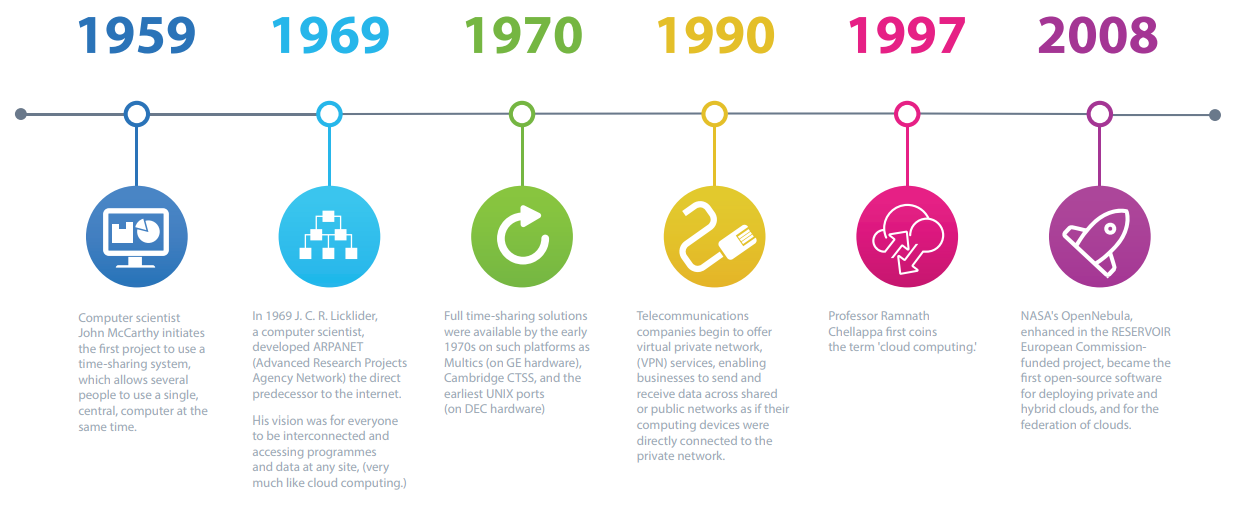
\includegraphics[width=1\textwidth]{lineacloud}
		\caption{Linea de tiempo de Cloud Computing}
		\label{fig:lineacloud}
	\end{center}
\end{figure}
\subsection{El modelo de entrega de IS}
\begin{justify}
La provisión de recursos de TI en las empresas está estrechamente vinculada con la consideración general de si la tecnología de la información y la comunicación debe mantenerse en la empresa o ser obtenida de proveedores externos -una cuestión que se establece en la investigación de la administración de empresas. En los últimos años, la opción de externalizar los servicios de TI a un proveedor de servicios externos ha crecido en importancia, debido a las ventajas de costo, calidad, flexibilidad y competencia. \cite{Markus}
\end{justify}
\subsubsection{Cloud computing como una evolución del outsourcing}
\begin{justify}
Aunque el outsourcing ha sido un tema establecido desde hace décadas y el núcleo del concepto todavía está alrededor de la cuestión duradera del aprovisionamiento de TI, el foco de la cuestión ha cambiado bastante con el tiempo. Al inicio del fenómeno de outsourcing se ha centrado la atención en la decisión entre una prestación interna o externa de servicios de TI y el tema de la subcontratación (infraestructura, aplicaciones y procesos), como se observa en la Figura \ref{fig:provisionTI}. La eficiencia de la subcontratación fue muy difícil de probar lo que dio lugar a un retroceso hacia la insourcing o backsourcing.
A pesar de las críticas, el concepto organizativo de outsourcing ha sido establecido y hoy en día los parámetros de diseño de un proyecto exitoso de outsourcing son de interés.
\end{justify}
\begin{figure}[ht]
	\begin{center}
		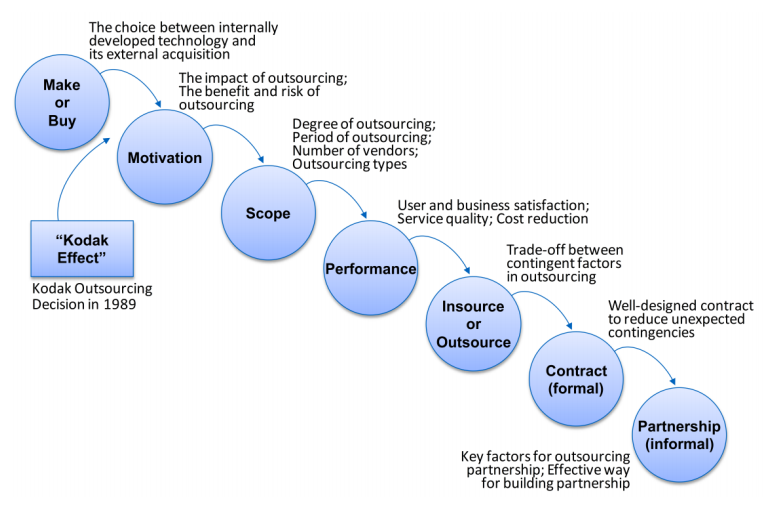
\includegraphics[width=1\textwidth]{provisionTI}
		\caption{Evolución del Outsourcing}
		\label{fig:provisionTI}
	\end{center}
\end{figure}
\subsubsection{Una comparación de la cadena de valor}
\begin{justify}
Una cadena de valor no sólo contiene diferentes empresas, sino también diferentes unidades de negocio dentro de una organización que producen conjuntamente un producto o servicio. El proceso de fabricación rara vez es estrictamente lineal y, por lo tanto, a menudo no se ve como una cadena de valor, sino como una red de valor. Es una red de relaciones que genera valor económico y otras ventajas a través de intercambios dinámicos complejos entre empresas. Especialmente con respecto a los nuevos servicios de Internet, las redes de valor se entienden a menudo como una red de proveedores, distribuidores, proveedores de servicios comerciales y clientes vinculados a través de Internet y otros medios electrónicos para crear valores para sus clientes finales \cite{Tapscott}.
\end{justify}
	\begin{enumerate}[label=\alph*)]
		\item{Cadena de valor de Outsourcing de servicios de TI tradicional: }
			En el outsourcing tradicional, la cadena de valor suele estar dividida en las áreas de infraestructura, aplicaciones y procesos de negocio, que pueden complementarse con estrategias y actividades de consultoría. En cada uno de estos cuatro pasos de cadena de valor se debe apoyar e implementar todo el ciclo de servicios de TI, a menudo denominado "planificar, construir y ejecutar". Por lo tanto, los aspectos individuales de los pasos individuales de la cadena de valor pueden ser subcontratados, como el desarrollo de aplicaciones. Compras y operación de hardware de TI, así como alojamiento puede ser dividido en los servicios que se realizan por el propio cliente y que utilizan los recursos de un proveedor de alojamiento. Aquí, las innumerables posibilidades de combinación pueden conducir a complejas relaciones de subcontratación. Esto se puede observar en la Figura \ref{fig:cadenaTradicional}
\begin{figure}[ht]
	\begin{center}
		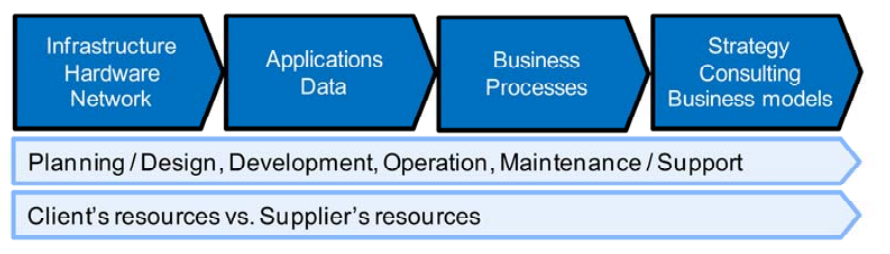
\includegraphics[width=1\textwidth]{cadenaTradicional}
		\caption{Cadena de valor del Outsourcing de Servicios de TI tradicional}
		\label{fig:cadenaTradicional}
	\end{center}
\end{figure}
		\item{Cadena de valor de Cloud Computing: }
		Se puede observar una tendencia general de los productos a los servicios. La tendencia no sólo conduce a una mayor externalización, sino también de la clásica subcontratación basada en hardware de centros de datos a la informática como servicio. Una tendencia similar se puede encontrar en el negocio de software. La computación en nube enlaza estas dos áreas de un outsourcing de hardware orientado a servicios más fuerte al concepto "como un servicio" para software. Aquí, la computación en nube muestra dos grandes facetas: los servicios basados en infraestructura ahora se ofrecen dinámicamente a las necesidades de los clientes, a menudo se refiere como la computación de servicios públicos.
En segundo lugar, surgieron nuevas plataformas de computación en nube, para integrar ofertas de hardware y software como servicio. Estas plataformas permiten crear aplicaciones y servicios nuevos, sencillos y compuestos que soportan procesos complejos e interconectan múltiples fuentes de datos. 
Al mirar estas plataformas desde una perspectiva de cadena de valor, pueden ser percibidas como una especie de mercado, donde se integran y se ofrecen al cliente diversos recursos de cloud computing de diferentes niveles (infraestructura, servicios de plataforma y aplicaciones). Mediante la composición de diferentes servicios, complejos procesos de negocio y puede ser apoyado y accedido a través de una interfaz de usuario unificada. El concepto de servicio en la nube de cloud computing permite desarrollar nuevas aplicaciones orientadas a servicios complejas que consisten en una mezcla de servicios tanto locales como fuera de las instalaciones, así como aplicaciones de nube pura. 
Podemos derivar tres actores principales dentro de la red de valor: el proveedor de servicios, el proveedor de la plataforma y el proveedor de infraestructura. El proveedor de infraestructura suministra a la red de valor todos los servicios de computación y almacenamiento necesarios para ejecutar aplicaciones dentro de la nube.
El proveedor de la plataforma ofrece un entorno en el que se pueden implementar las aplicaciones de la nube. También actúa como una especie de catálogo o mercado en el que las aplicaciones se ofrecen al cliente a través de un simple portal. El proveedor de servicios desarrolla aplicaciones que se ofrecen e implementan en la plataforma de cloud computing. Como queremos destacar especialmente el aspecto de la composición del servicio, hemos agregado el rol de agregador a la red simplificada de valor de computación en nube representada en la Figura \ref{fig:cadenaCloud}
		
\begin{figure}[ht]
	\begin{center}
		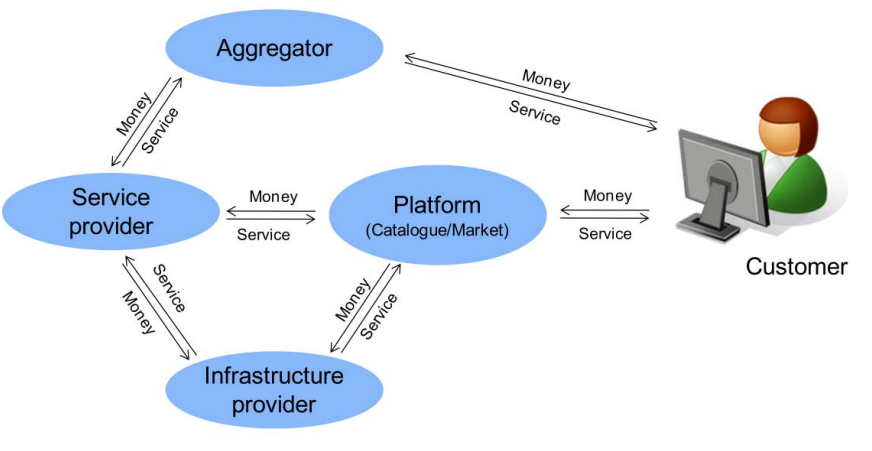
\includegraphics[width=1\textwidth]{cadenaCloud}
		\caption{Cadena de valor de Cloud}
		\label{fig:cadenaCloud}
	\end{center}
\end{figure}
	\end{enumerate}
\section{Concepto De La Computaci\'on Cloud}
\begin{justify}
Una definici\'on para la Computaci\'on Cloud es que puede ser visto como un sistema de computaci\'on distribuido orientado al consumidor. Dicho sistema consiste en una agrupaci\'on de ordenadores virtualizados e interconectados que son suministrados din\'amicamente y presentados como uno o m\'as recursos computacionales unificados.
\end{justify}
\section{Caracter\'isticas De La Computaci\'on Cloud}
\begin{justify}
No es necesario disponer de un equipo potente, tan s\'olo de un aparato con conexi\'on a internet; esto debido a que el dispositivo del usuario no realizar\'ia ning\'un proceso complejo y los ficheros pueden guardarse en la nube. Los servidores en donde se hallan los programas que se utilicen son los encargados de las tareas complicadas que antes se realizaba localmente.
\end{justify}
Algunas caracter\'isticas de la Computaci\'on Cloud, seg\'un \cite{oscarAvilaMejia}, son:
\begin{itemize}
    \item{Escalabilidad:} El sistema establece un nivel de servicios que crea nuevas instancias de acuerdo a la demanda de operaciones existente de tal forma que se reduzca el tiempo de espera y los cuellos de botella.
    \item{Virtualizaci\'on:} Las aplicaciones son independientes del hardware en el que corran. El usuario es libre de usar la plataforma que desee en su terminal (Windows, Unix, Mac, etc.), al utilizar las aplicaciones existentes en la nube puede estar seguro de que su trabajo conservar\'a sus caracter\'isticas bajo otra plataforma.
    \item{Autoreparable:} En caso de surgir un fallo, el \'ultimo respaldo (backup) de la aplicaci\'on se convierte autom\'aticamente en la copia primaria y a partir de \'esta se genera uno nuevo.
    \item{Seguridad:} El sistema permite a diferentes clientes compartir la infraestructura sin preocuparse de comprometer su seguridad y privacidad; de esto se ocupa el sistema proveedor que se encarga de cifrar los datos.
    \item{Disponibilidad:} No se hace necesario guardar los documentos del usuario en su computadora o en medios f\'isicos ya que la informaci\'on radicar\'a en Internet permitiendo su acceso desde cualquier dispositivo conectado a la red.
    \item{Precios:} La computaci\'on cloud no requiere una inversión adicional. No se requiere ning\'un gasto de capital. Los usuarios pagan por servicios y capacidad cuando los necesitan.
\end{itemize}
\section{Clasificaci\'on De Las Soluciones Computaci\'on Cloud}
\subsection{Seg\'un Modelos De Servicio}
\begin{justify}
La computación en nube puede ser vista como una colección de servicios, la cual puede ser presentada como una arquitectura en capas, como se muestra en la figura \ref{fig:capas1}:
\begin{figure}[ht]
	\begin{center}
		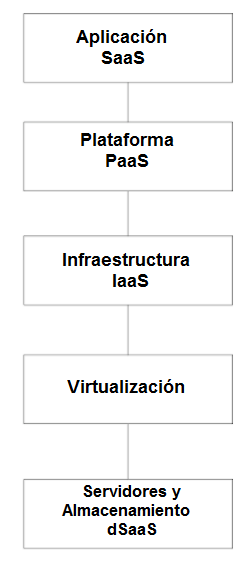
\includegraphics[width=.3\textwidth]{cloudcapas}
		\caption{Arquitectura en capas de computaci\'on cloud \cite{handbook}}
		\label{fig:capas1}
	\end{center}
\end{figure}
\begin{enumerate}[label=\alph*)]
    \item{IaaS:} Se refiere a los recursos informáticos como un servicio. Esto incluye computadoras virtualizadas con potencia de procesamiento garantizada y ancho de banda reservado para almacenamiento y acceso a Internet
    \item{PaaS:} Es similar a IaaS, pero también incluye sistemas operativos y servicios requeridos para una aplicación particular. En otras palabras, PaaS es IaaS con un stack de software personalizado para la aplicación dada.
    \item{SaaS:} Que se muestra en la parte superior de la figura \ref{fig:capas1}. SaaS permite a los usuarios ejecutar aplicaciones de forma remota desde la nube.
    \item{dSaaS:} Proporciona almacenamiento que el consumidor utilizar\'a, incluyendo los requisitos de ancho de banda para el almacenamiento.
\end{enumerate}
\end{justify}

\subsection{Seg\'un Tipo De Nube}
\begin{justify}
Hay tres tipos de computación cloud, los cuales se muestran en la figura \ref{fig:cloudtipos}
\begin{figure}[ht]
	\begin{center}
		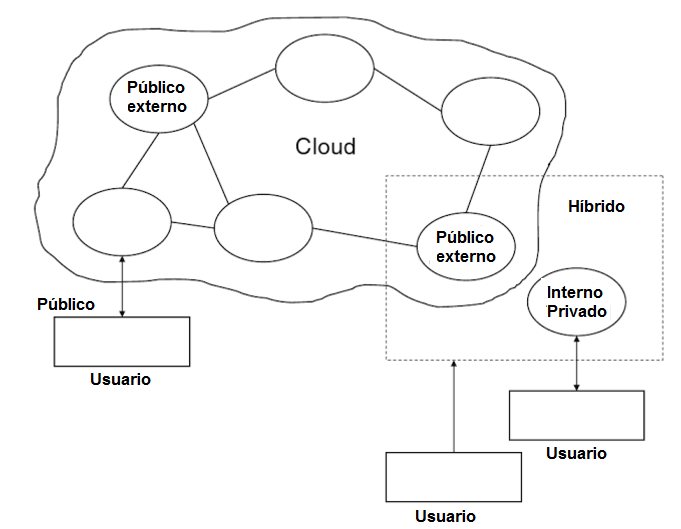
\includegraphics[width=.8\textwidth]{cloudtipos}
		\caption{Tres tipos de computaci\'on cloud \cite{handbook}}
		\label{fig:cloudtipos}
	\end{center}
\end{figure}
\begin{enumerate}[label=\alph*)]
    \item{P\'ublica:} En la nube pública (o en la nube externa), los recursos inform\'aticos se suministran din\'amicamente mendiante Internet a trav\'es de aplicaciones Web o Servicios Web de un proveedor externo (de terceros). Las nubes p\'ublicas son ejecutadas por terceros, y es probable que las aplicaciones de diferentes clientes se mezclen entre sí en los servidores, sistemas de almacenamiento y redes de la nube.
    \item{Privada:} La nube privada (o nube interna) se refiere a la computaci\'on cloud en redes privadas. Las nubes privadas se construyen para el uso exclusivo de un cliente, proporcionando un control total sobre los datos, la seguridad y la calidad del servicio. Las nubes privadas pueden ser construidas y administradas por la propia organización de TI de la empresa o por un proveedor de la nube.
    \item{H\'ibrida:} Un entorno de nube híbrido combina los modelos de nube pública y privada. Las nubes híbridas introducen la complejidad de determinar cómo distribuir aplicaciones a través de una nube pública y privada
    \item{Comunitaria:} El modelo de nube comunitaria permite el acceso a un número de organizaciones o consumidores que pertenecen a una comunidad y el modelo se construye para servir a algún propósito común y específico. Es para el uso de alguna comunidad de personas u organizaciones que comparten preocupaciones comunes en funcionalidades empresariales, requisitos de seguridad, etc. Este modelo permite compartir infraestructura y recursos entre múltiples consumidores pertenecientes a una única comunidad y por lo tanto se hace más barato comparado con una nube privada \cite{sandeep}
\end{enumerate}
\end{justify}

\subsection{Según Por Agentes Intervinientes En El Negocio}
\begin{justify}
Los agentes intervinientes en el negocio seg\'un \cite{tratecno}, se muestran en la figura \ref{fig:agentesintervinientes}
\begin{figure}[ht]
	\begin{center}
		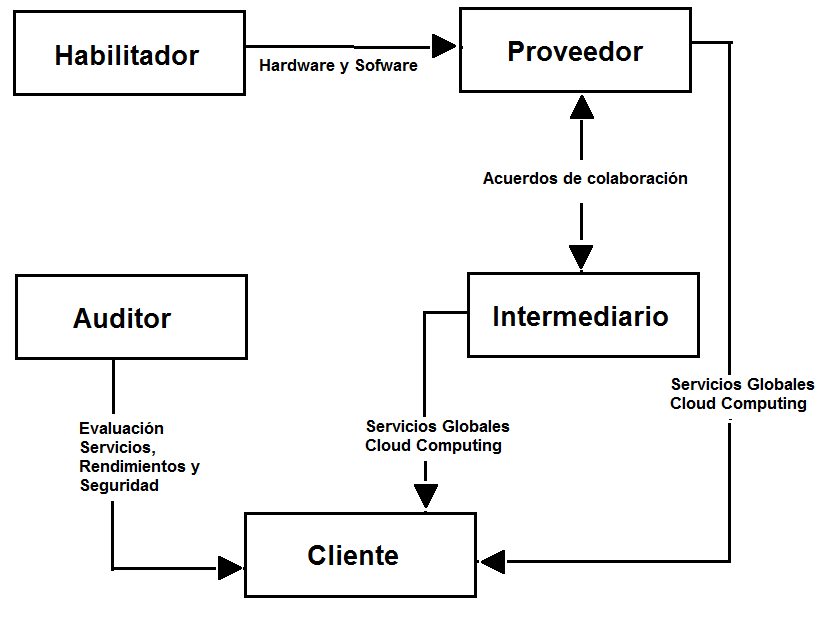
\includegraphics[width=.6\textwidth]{agentesintervinientes}
		\caption{Agentes intervinientes en el negocio \cite{tratecno}}
		\label{fig:agentesintervinientes}
	\end{center}
\end{figure}
\begin{enumerate}[label=\alph*)]
    \item{Habilitador:} Enfocados a ofrecer una serie de servicios Hardware o Software a otros proveedores.
    \item{Proveedor:} Los servicios que presta a los intermediarios y clientes, o bien los genera directamente el, o los contrata a otros proveedores o habilitadores.
    \item{Auditor:} Las funciones a desarrollar por los auditores, son las de llevar a cabo evaluaciones de los servicios, rendimientos y seguridad de las operaciones en el uso de las soluciones Cloud.
    \item{Intermediario:} Los intermediarios adecuan las soluciones para los clientes negociando los distintos servicios, añadiéndole en muchos casos ciertos servicios adicionales como pueden ser algunos apoyos en formación, implementación, etc.
    \item{Cliente:} Dentro del esquema de los agentes intervinientes, es aquel que va a contratar los servicios del resto de los agentes.
\end{enumerate}

\end{justify}

%%%%%%%%%%%%%%%%%%%%%%%%%%%% CAPITULO 2 %%%%%%%%%%%%%%%%%%%%%%%%%%%%
\vspace*{5em}
\chapter{VENTAJAS, DESVENTAJAS Y RETOS}
\vspace*{-2em}
\section{Ventajas}
\begin{justify}
Las soluciones y servicios de cloud computing ofrecen una serie de ventajas a las empresas privadas (econ\'omico-financieras,foco en el negocio, rapidez y flexibilidad, tecnol\'ogicas, seguridad, disponibilidad y movilidad, etc.), a la econom\'ia, a las organizaciones p\'ublicas y de investigaci\'on y a los ciudadanos (mayor y mejor oferta de servicios, gobierno abierto, educaci\'on), respecto de las funcionalidades ofrecidas por los sistemas tradicionales de TI y esto es gracias a su rapidez, flexibilidad, disponibilidad, etc. De entre todas las ventajas que hay, las más notables para los usuarios son el ahorro en costes y la facilidad para aumentar los recursos disponibles.
\\ Los ahorros en costes son debidos a que es posible evitar los gastos tanto en hardware, como en software, soporte y seguridad. Por otro lado, la flexibilidad y la escalabilidad de los recursos se hace de una manera muy sencilla y en el momento que el cliente lo requiera, de forma que puede aumentar o disminuir los recursos que está utilizando en cualquier momento y adem\'as pagando solo por lo que usa. Otra de las ventajas m\'as atrayentes es la capacidad de recuperación ante problemas, o desastres.
\\ Podemos decir que gracias a todas las ventajas que ofrece el paradigma del cloud computing frente a los m\'etodos tradicionales, est\'a haciendo que aumente la productividad de las empresas, se mejore en los servicios públicos y la calidad de vida.

\end{justify}
\newpage
\subsection{Ventajas para las empresas}
\begin{justify}
Actualmente el cloud computing es un instrumento acelerador para que una empresa logre evolucionar en su competividad proporcionando ventajas estrat\'egicas, t\'ecnicas, para la sostenibilidad y econ\'omicas que ya se mencionaron antes.
\begin{enumerate}[label=\alph*)]
    \item{Ventajas estrat\'egicas:} 
				\begin{itemize}
						\item{Creaci\'on de nuevos productos y servicios: } Esto es posible debido a la reduccio\'n de 	costes, que hace que sea posible que las empresas creen nuevos productos y/o servicios, que antes no resultaban rentables.
						\item{Trabajo colaborativo: } La computaci\'on en la nube permite que muchas personas a la vez puedan trabajar sobre la misma herramienta, aplicaci\'on o documento, de esta manera se fomenta la productividad, comunicaci\'on y colaboraci\'on entre empleados.
						\item{Mejora de la productividad: } Como los recursos est\'an disponibles para acceder a ellos desde cualquier ubicaci\'on f\'isica, se puede trabajar sobre los recursos de forma online, desde cualquier lugar, haciendo que aumente la flexibilidad de la empresa para trabajar a distancia y la productividad de sus empleados.
						\item{Innovaci\'on: } El ahorro en costes hace que la empresa pueda centrar sus esfuerzos en desarrollar su activadad de negocio, haciendo posible que la empresa tenga m\'as posibilidades de invertir en innovaci\'on.
				\end{itemize}
		\newpage
    \item{Ventajas te\'cnicas:}
				\begin{itemize}
						\item{}La nube es una plataforma que permite a los usuarios disponer de la tecnolog\'ia m\'as actual, lo que hace que no haya riesgo de p\'erdida de competitividad por obsolescencia tecnol\'ogica. Adem\'as de esto el tiempo de adopci\'on de nuevos servicios, infraestructuras o tecnolog\'ias es mucho menor. 
						\item{}Los proveedores de cloud computing tambi\'en ofrecen soporte y redundancia en los sistemas que sus clientes contratan, de manera que existe una gran resistencia a desastres y buena capacidad de recuperación ante fallos.
				\end{itemize}
    \item{Ventajas para la sostenibilidad:} 
				\begin{itemize}
						\item{}La reducción en el consumo de energ\'ia es notable, debido a que la empresa necesita de menos equipamiento propio, ya que lo contrata al proveedor. Esto es posible porque la empresa no dispone de un exceso de recursos inform\'aticos, sino que la plataforma que contrata se adapta a las necesidades de su entidad. Los centros de datos utilizan diseños de infraestructuras avanzados, de forma que los sistemas de refrigeraci\'on y de acondicionamiento de energ\'ia se aprovechen bien y no haya p\'erdidas.
				\end{itemize}
\end{enumerate}
\end{justify}
\newpage
\subsection{Ventajas para la econom\'ia}
\begin{justify}
El cloud computing genera un notable efecto de dinamizaci\'on econ\'omica y del empleo en aquellos pa\'ises en los que su desarrollo e implantaci\'on est\'a m\'as evolucionado. Al igual que el sector TIC o la aparici\'on de Internet gener\'o una revoluci\'on de los modelos empresariales y econ\'omicos durante las tres \'ultimas d\'ecadas y supuso un motor de desarrollo para todos los pa\'ises, el cloud computing est\'a llamado a ser un nuevo punto de ruptura para la econom\'ia mundial en general y para el sector de las tecnolog\'ias y servicios profesionales en particular.
\\ Este efecto dinamizador se fundamenta en el hecho de que los beneficios que obtienen las empresas proveedoras de servicios cloud se reinvierte en la econom\'ia a trav\'es de consumos intermedios en otros sectores derivados, genera una dinamizaci\'on de empleo cualificado e incrementa el poder adquisitivo y el consumo en un territorio. 
\\ Adicionalmente, las empresas suscriptoras del servicio adquieren las econom\'ias de escala de los proveedores, reduciendo con ello sus costes globales en TI. Gracias a la presencia de estas econom\'ias de escala en el sector, se suprimen las barreras de entrada en el mercado de nuevos proveedores, suscriptores e intermediarios, dinamizando la econom\'ia y promoviendo la aparición de nuevos modelos de negocio, productos y servicios y facilitando la creación de nuevas empresas y empleo.
\\ Estas econom\'ias de escala también favorecen la sostenibilidad de las empresas de nueva creación que pueden dedicar todos sus esfuerzos a su negocio y reducir el riesgo de "morir de \'exito"\hspace{0.1cm}por no poder escalar adecuadamente ante situaciones de demanda superior a las expectativas. Es evidente que esta ventaja resulta de especial trascendencia para las pequeñas y medianas empresas.
\\ Adicionalmente, la mayor eficiencia en el uso de la infraestructura TI permite ahorros energ\'eticos significativos con la consiguiente mejora en el impacto medioambiental, añadiendo a los atractivos de las tecnolog\'ias cloud computing el de ser respetuosas con el medio ambiente

\end{justify}
\newpage
\subsection{Ventajas para las administraciones p\'ublicas}
\begin{justify}
Una administraci\'on p\'ublica es similar en muchos aspectos a una empresa privada, ya que ambas lo que buscan es prestar servicios, gestionar recursos, relacionarse con los proveedores, etc. Entonces, es lógico pensar que estas entidades tambi\'en pueden optar por una soluci\'on cloud para desempeñar su actividad y as\'i beneficiarse de las ventajas que ofrece esta tecnolog\'ia.

Adem\'as de las ventajas obvias que este paradigma aporta a este tipo de entidades, tales como el ahorro en costes tecnol\'ogicos, la flexibilidad y la escalabilidad, el ahorro energ\'etico, existen otras muchas ventajas espec\'ificas para las administraciones p\'ublicas:
				\begin{itemize}
						\item{}Facilita las tareas de soporte tecnol\'ogico intensivo, ya que es el proveedor el que se encarga de esto y por lo tanto no se incurre en grandes gastos en este aspecto.
						\item{}Generalizaci\'on de todos los servicios transversales de la Administraci\'on y por lo tanto un aprovechamiento y reutilizaci\'on de las infraestructuras tecnol\'ogicas.
						\item{}Modernizaci\'on de entidades pequeñas, locales o municipales, que no disponen
de recursos necesarios para modernizar sus procesos y equipos de la forma tradicional.
						\item{}Investigaci\'on y colaboraci\'on en entidades con car\'acter educativo, tales como universidades, fundaciones, centros de investigaci\'on, etc. Incluso la cooperaci\'on entre estos centros.
				\end{itemize}
\end{justify}
\newpage
\subsection{Ventajas para la investigaci\'on cient\'ifica}
\begin{justify}
Es totalmente esencial que exista un ambiente de colaboraci\'on e interoperabilidad entre entidades dedicadas a la investigaci\'on, adem\'as de la existencia de tecnolog\'ias avanzadas, por lo que la nube, tanto privada como p\'ublica, puede favorecer en muchos aspectos al desarrollo de estas actividades.
Algunas de las ventajas m\'as notables del cloud computing en estas \'areas son las siguientes:
				\begin{itemize}
						\item{}Plataformas de colaboraci\'on entre entidades, de manera que la realizaci\'on de investigaciones y proyectos de forma conjunta es mucho m\'as r\'apida y eficaz.
						\item{}Estandarizaci\'on de sistemas, procesos y datos entre empresas que participan
en el mismo proyecto.
						\item{}Disposici\'on de entornos grandes e intensivos de procesamiento de datos, de manera que las tareas se realicen m\'as ágilmente y ahorrando en costes.
				\end{itemize}
\end{justify}
\newpage
\subsection{Ventajas para los ciudadanos}
\begin{justify}
Gracias a la tecnolog\'ia cloud ahora es posible acceder a la informaci\'on desde cualquier localizaci\'on.Las caracter\'isticas de este paradigma no son visibles para los usuarios, pero gracias a ellas, son capaces de acceder a gran variedad de servicios de forma gratuita o a precios muy bajos y lo m\'as importante, sin necesidad de disponer de equipos especializados para ello. Algunos de estos servicios más t\'ipicos y conocidos son los gestores de correo electr\'onico, buscadores, enciclopedias, \'albumes de fotograf\'ias, etc.
Entre las principales ventajas para los ciudadanos, que aporta la computaci\'on cloud tenemos:
				\begin{itemize}
						\item{}Amplia oferta de servicios y productos tecnol\'ogicos similares, debido a la competitividad existente, que permite a los ciudadanos poder elegir entre las soluciones que le parecen m\'as estables, econ\'omicas y seguras.
						\item{}Variedad en los servicios disponibles para que los ciudadanos realicen sus tareas cotidianas, desde ocio, hasta trabajo, gesti\'on del hogar, educaci\'on, etc. Gracias a los dispositivos m\'oviles, la utilizaci\'on de estos servicios es mucho m\'as sencilla.
						\item{}Los ciudadanos pueden acceder a un mayor n\'umero de servicios, gracias a la administración electr\'onica. Lo hacen a trav\'es de Internet y de esta forma pueden realizar de manera m\'as sencilla, \'agil y efectiva muchos tr\'amites de la administraci\'on.
						\item{}Disponibilidad de un "gobierno abierto"\hspace{0.1cm}que permita que los ciudadanos puedan acceder a la informaci\'on sobre las actividades realizadas por el gobierno, sus gastos, datos que genera, etc. Además de fomentar la participaci\'on ciudadana para diseñar pol\'iticas p\'ublicas.
						\item{}Las redes sociales permiten que los ciudadanos compartan experiencias, conocimientos, que hagan negocios o que demanden bienes y servicios.
				\end{itemize}
\end{justify}
\newpage
\section{Desventajas}
\begin{justify}
Junto a los beneficios tambi\'en existen ciertas desventajas o riesgos expuestos por los
detractores de esta tecnolog\'ia y que nos recomiendan no confiar toda la informaci\'on de nuestra empresa a la Nube.
Entre las principales desventajas tenemos:
				\begin{itemize}
						\item{}El problema de la estabilidad de la conexi\'on a Internet. Los detractores dudan de que la velocidad de conexi\'on y la estabilidad proporcionada por los ISP sea suficiente para gestionar el volumen de datos generado por el n\'umero de empresas que se sumen a la Nube. 
						\item{} Tener nuestra informaci\'on y su gesti\'on a la Nube significa perder el control sobre ella y si el proveedor de servicios de la Nube tiene un problema a la hora de suministrar, \'este se traduce autom\'aticamente en la imposibilidad de acceder a nuestros datos y, por tanto, de trabajar. Si el tiempo es oro para nuestro negocio, confiar en la Nube puede ser lo menos aconsejable.

						\item{}Otro problema es el de la seguridad. Por ejemplo, aquella informaci\'on extremadamente confidencial o delicada y que se encuentre en la Nube en manos de terceros en quienes confiamos que hagan un buen trabajo a la hora de asegurarla y protegerla, pero si no es as\'i, los grandes perjudicados seremos nosotros, lo mismo se puede aplicar para aquella información privada de los empleados de una empresa. Hoy en d\'ia se esta acostumbrado a que los empleados usen los recursos de la empresa (Servidores, conexi\'on a Internet, etc.) para gestiones privadas y esa misma privacidad podr\'ia ser amenazada si esos datos se encuentran almacenados en un sitio controlado por otros. 
				\end{itemize}
				
En definitiva, debemos reflexionar tanto las ventajas como las desventajas y compararlas con las necesidades espec\'ificas del negocio actual. Si nos preocupa sobre todo el presupuesto, la Nube puede ser una buena opci\'on a considerar; pero si, por el contrario, nuestra mayor preocupaci\'on es la seguridad y protecci\'on de nuestra informaci\'on, la Nube está todavía muy lejos de ser considerada como alternativa viable.
\newpage
El volumen de datos tambi\'en es un delimitador para saber si una pequeña o mediana empresa est\'a preparada para ser elevada a la Nube. Cuanto mayor sea el volumen de informaci\'on que procesamos y
almacenamos, menos recomendable será confiar en la computación en nube. Algunas soluciones intermedias podria ser subir a la Nube s\'olo una parte de nuestra informaci\'on; aquella, por ejemplo, que precise ser accesible desde m\'ultiple localizaciones. Y el resto, la m\'as sensible, almacenarla y gestionarla desde sistemas propios.
\end{justify}
\newpage
\section{Retos}
\begin{justify}
Los principales retos del cloud computing están relacionados con la seguridad, m\'as concretamente con la confindencialidad y privacidad de los datos y con la disponibilidad e integridad de los servicios y los datos.

Seg\'un la Universidad de Berkley, existen diez retos a los que se enfrenta el cloud computing y son los siguientes:
				\begin{itemize}
						\item{}Disponibilidad del servicio
						\item{}Bloqueo de los datos
						\item{}Confidencialidad de los datos y auditabilidad
						\item{}Cuellos de botella en la transferencia de datos
						\item{}Rendimiento del servicio impredecible
						\item{}Escalabilidad de la capacidad de almacenamiento
						\item{}Tolerancia a fallos en sistemas distribuidos a gran escala
						\item{}R\'apida escalabilidad tecnológica
						\item{}Prejuicio de reputaci\'on
						\item{}Licencias de software
				\end{itemize}
A continuación, en las siguientes secciones, vamos a explicar algunos de los
retos más notables que afectan a este paradigma.
\end{justify}
\newpage
\subsection{Disponibilidad del servicio}
\begin{justify}
Como se trata de una tecnolog\'ia emergente, existen dudas sobre si el proveedor ser\'a capaz de cumplir los niveles de servicio acordados en todo momento. Sobre todo en los procesos m\'as cr\'iticos para el cliente. Para subsanar estas dudas o problemas, hay que analizar el impacto que la pérdida de servicio pueda suponer y buscar alternativas. Además, en los acuerdos se pueden fijar cl\'ausulas de penalizaci\'on.
\end{justify}
\subsection{Restricciones geogr\'aficas}
\begin{justify}
Los servicios de cloud pueden ser proporcionados a trav\'es de geografías diferentes. Por ello, las entidades p\'ublicas y privadas deben ser conscientes de situaciones excepcionales relativas a la  ubicación f\'isica, tales como leyes y regulaciones locales, que puedan afectar en temas de privacidad, seguridad y protecci\'on de datos de car\'acter personal y confidencial.
\end{justify}
\subsection{Seguridad y privacidad de datos}
\begin{justify}
Los datos residen en sistemas tecnol\'ogicos que se encuentran fuera del alcance del firewall de la empresa. Por este motivo, existe una gran resistencia al uso de la tecnolog\'ia cloud en las empresas privadas y organizaciones p\'ublicas, en los sistemas de la entidad que contienen informaci\'on cr\'itica para la misma.

Adem\'as de esto, dependiendo del tipo de datos que maneje la empresa, el lugar de desarrollo de su actividad, etc, es necesario tener en cuenta la Ley Org\'anica de Protecci\'on de Datos. Esta ley, establece las medidas que hay que tomar a la hora de tratar con datos de car\'acter personal. As\'i como aspectos de transferencia internacional de datos, subcontrataci\'on, derechos ARCO, etc.
\end{justify}
\newpage
\subsection{Amortizaci\'on tecnol\'ogica}
\begin{justify}
Las empresas y organizaciones p\'ublicas han invertido muchos recursos durante las \'ultimas d\'ecadas en implementar procesos de modernizaci\'on tecnol\'ogica e inversi\'on en infraestructuras y personal para el \'area de TI. La utilizaci\'on del cloud puede generar ciertas dudas para los directores de \'areas de sistemas que todav\'ia cuentan con activos tecnol\'ogicos no amortizados y que han logrado configurar un equipo de trabajo estable y cualificado para su administraci\'on. Aunque es indudable que cloud puede generar un punto de ruptura en las estrategias de sistemas ya establecidas, su adopci\'on debe ser considerada como algo progresivo, planificado y sostenible, estableciendo procesos de migraci\'on paulatinos y controlables que permitan garantizar la adecuada amortizaci\'on y sustituci\'on de los activos actuales y reorientar al personal de TI hacia l\'ineas de trabajo de valor para el departamento.
\end{justify}
%%%%%%%%%%%%%%%%%%%%%%%%%%%% CAPITULO 3 %%%%%%%%%%%%%%%%%%%%%%%%%%%%
\vspace*{5em}
\chapter{COMPUTACI\'ON CLOUD EN LA ACTUALIDAD 3}
\vspace*{-2em}
\begin{justify}
La nube es actualmente, no solo una soluci\'on a m\'ultiples problem\'aticas empresariales, sino tambi\'n una tendencia principal en las estrategias de negocio debido a su escalabilidad, adaptabilidad y flexibilidad y en la forma en como eficiente la monetizaci\'on en las compa\~n\'ias y en como tambi\'en democratiza el acceso a la tecnolog\'ia.\par

Con la acelerada transformaci\'on de las tecnolog\'ias de la informaci\'on (TI), la nube se ha convertido en una herramienta para la supervivencia de diversas empresas de diferentes tama\~nos, esto debido a que ayuda a crear nuevas soluciones, conectar aplicaciones, optimizar el recurso adecuado en el momento adecuado y poder as\'i responder a las demandas del mercado.
Sin embargo, a pesar de contar con todos los beneficios, mencionados anteriormente, que tiene implementar una estrategia de nube, existen empresas que están retrasando la decisión de adoptarla poniendo as\'i en riesgo el quedarse atr\'as en una transformaci\'on digital que exige con mucha premura la competitividad.\par

Para conocer mejor la situaci\'on actual de la nube en las empresas revisaremos los resultados obtenidos de la encuesta CloudView realizada en el 2016 por la IDC (International Data Corporation). Para esta encuesta se entrevist\'o a personas que participan en la toma de decisiones de TI, de una muestra global de 11 350 ejecutivos la encuesta se realiz\'o a 6159, que utilizaban la nube de forma activa para m\'ultiples cargas de trabajo. Como vemos en la figura \ref{fig:perfilEncuesta} el 37\% de los encuestados pertenecen a Asia y el pac\'ifico, mientras que un 27\% pertenecen a Europa, Oriente Medio y \'Africa (EMEA) y aproximadamente un 36\% al continente americano, tambi\'en se puede apreciar que un poco menos de la mitad (43\%) de los encuestados son ejecutivos de alto nivel dentro de su empresa y por \'ultimo casi las tres cuartas partes (73\% aprox.) pertenec\'ian a medianas y grandes empresas. Al pie podemos apreciar las preguntas aplicadas durante la realizaci\'on de la encuesta.\par

\begin{figure}[ht]
	\begin{center}
		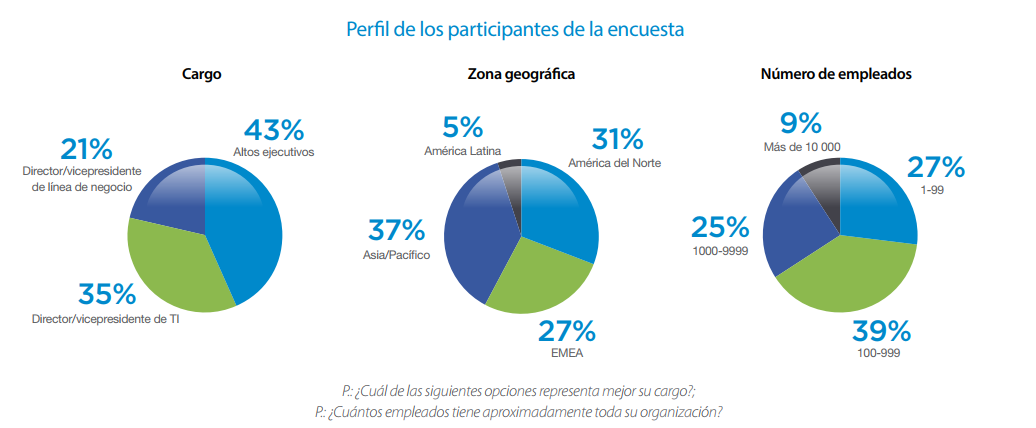
\includegraphics[width=.8\textwidth]{perfilEncuesta}
		\caption{Perfil de los participantes de la encuesta}
		\label{fig:perfilEncuesta}
	\end{center}
\end{figure}

Respecto al uso de las nubes, ya sea de tipo privada o p\'ublica, esta encuesta muestra que, como se puede observar en la figura \ref{fig:empresasYNubes}, el porcentaje de empresas que la utilizan es mayor respecto al año 2015, y así también se ha reducido el porcentaje que desconocen de este modelo, de un 19\% a un 10\%.  Esto nos indica que los beneficios logrados por las empresas que ya ten\'an implementada un tipo de nube han influenciado para que otras empresas se interesen en este modelo, se adapten y puedan ser competitivas dentro del mercado.\par

\begin{figure}[ht]
	\begin{center}
		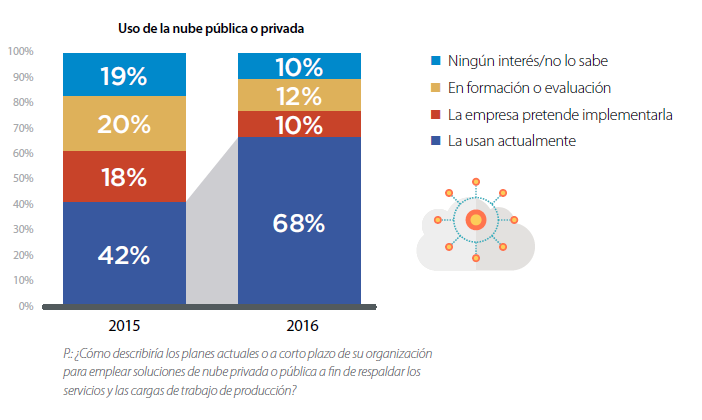
\includegraphics[width=.8\textwidth]{empresasYNubes}
		\caption{Empresas que utilizan un tipo de nube}
		\label{fig:empresasYNubes}
	\end{center}
\end{figure}

El tipo de nube que implemente una empresa depender\'a de los servicios que ofrezca, del presupuesto con el que cuente, entre otros aspectos, y como se muestra en la figura \ref{fig:adopcionDeLaNube}, la adopci\'on seg\'un la encuesta se divide de forma relativamente uniforme entre ambos tipos de nube.\par

\begin{figure}[ht]
	\begin{center}
		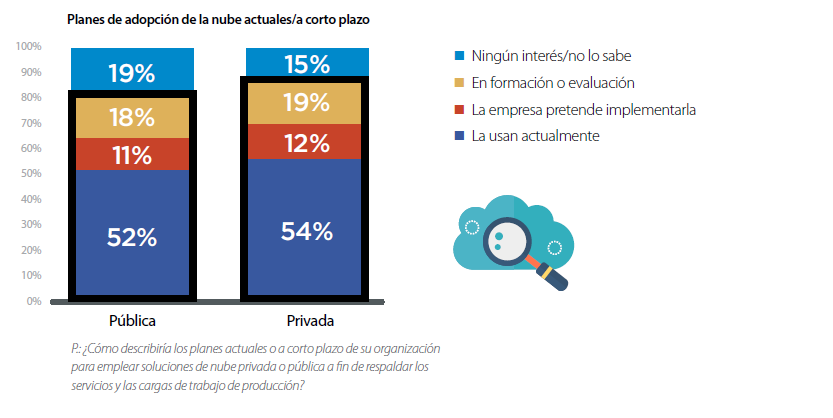
\includegraphics[width=.8\textwidth]{adopcionDeLaNube}
		\caption{Adopci\'on de la nube p\'ublica y privada}
		\label{fig:adopcionDeLaNube}
	\end{center}
\end{figure}

Sin embargo, se observa que la mayor\'ia de las personas o empresas que adoptan la nube utiliza m\'as bien alg\'un tipo de nube h\'ibrida (Figura \ref{fig:utlizacionDeNubesHibridas}), estamos hablando de que alrededor del 73\% tienen una estrategia de nube h\'ibrida y dentro de los cuales la suscripci\'on a servicios externos es la caracter\'istica m\'as adoptada.\par

\begin{figure}[ht]
	\begin{center}
		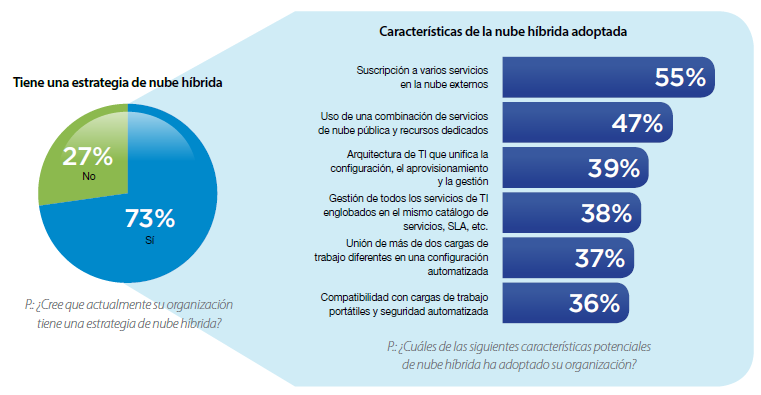
\includegraphics[width=.8\textwidth]{utlizacionDeNubesHibridas}
		\caption{Utilizaci\'on de nubes h\'ibridas y caracter\'isticas relevantes}
		\label{fig:utlizacionDeNubesHibridas}
	\end{center}
\end{figure}

Ahora bien, enfoc\'andonos un poco en los distintos tipos de implementac\'on de una nube privada dentro de las empresas, se observa que existen muchas organizaciones que utilizan m\'as de un tipo de implementaci\'on (Figura \ref{fig:planesImplementacionNube}).\par

\begin{figure}[ht]
	\begin{center}
		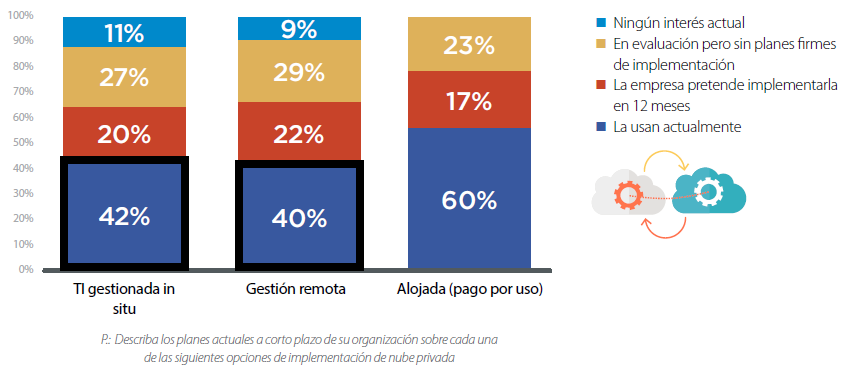
\includegraphics[width=.8\textwidth]{planesImplementacionNube}
		\caption{Planes de implementaci\'on de nube privada alojada}
		\label{fig:planesImplementacionNube}
	\end{center}
\end{figure}

IDC clasifica a las organizaciones en cinco niveles de adopci\'on de la nube, es decir dependiendo del nivel de uso que le den dentro de \'esta y de la calidad de servicios que ofrecen dichas organizaciones como resultado del uso de esta tecnolog\'ia se pueden clasificar como se muestra en la figura \ref{fig:clasificacionOrganizaciones} , donde se puede apreciar que un mayor uso de un tipo de nube sea p\'ublica o privada conlleva a una mejora en los servicios que ofrecen, posicion\'andose as\'i mejor en el mercado.\par

\begin{figure}[ht]
	\begin{center}
		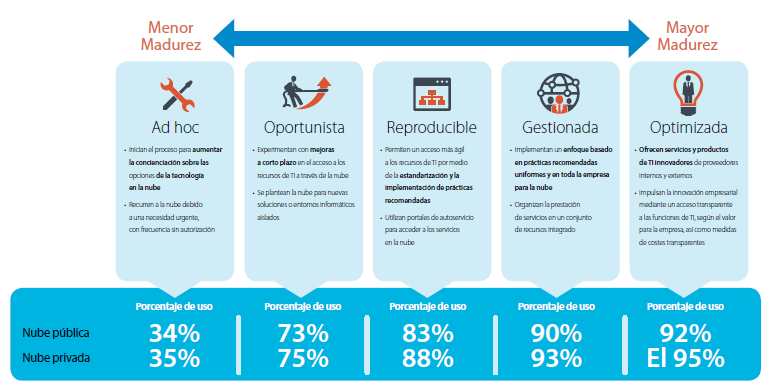
\includegraphics[width=.8\textwidth]{clasificacionOrganizaciones}
		\caption{Clasificaci\'on de las organizaciones seg\'un el nivel de adopci\'on de la nube}
		\label{fig:clasificacionOrganizaciones}
	\end{center}
\end{figure}

De acuerdo con la clasificaci\'on vista, en la figura \ref{fig:madurezNube} observamos la cantidad de organizaciones de acuerdo al nivel en el que se encuentran, teniendo as\'i que tan solo un 3\% se encuentran en el m\'as alto nivel y un 22\% a\'un se encuentran sin estrategia alguna, posiblemente porque esas organizaciones se resisten al cambio que implica implementar este modelo. Pero tambi\'en se observa que la mayor\'ia sigue intentando mejorar sus estrategias de nube.\par

\begin{figure}[ht]
	\begin{center}
		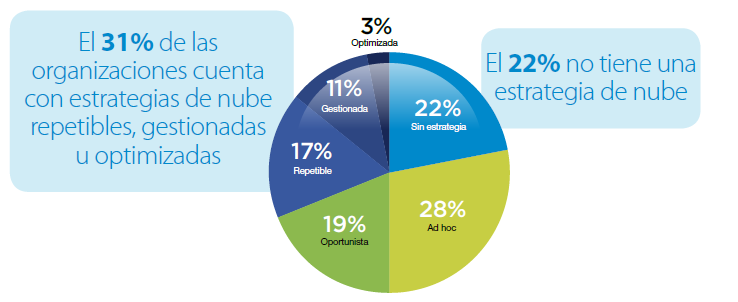
\includegraphics[width=.8\textwidth]{madurezNube}
		\caption{Nivel de madurez de la nube}
		\label{fig:madurezNube}
	\end{center}
\end{figure}

El que una organizaci\'on tenga un mayor nivel de madurez en su estrategia de nube le proporciona m\'ultiples ventajas como las mostradas en la figura \ref{fig:ventajasMadurezNube} .\par

\begin{figure}[ht]
	\begin{center}
		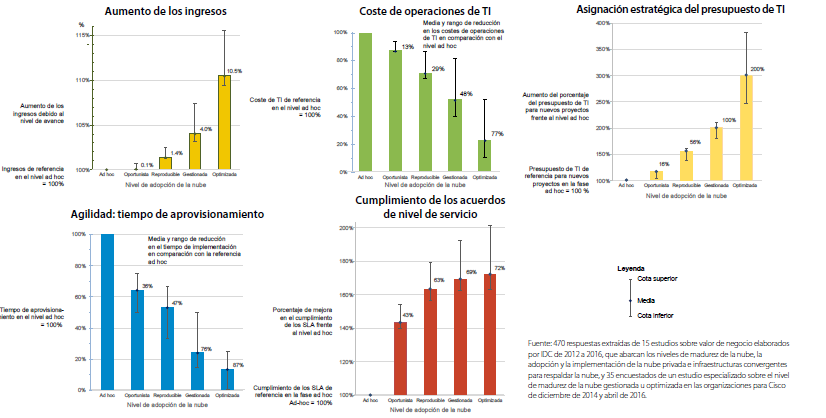
\includegraphics[width=.8\textwidth]{ventajasMadurezNube}
		\caption{Ventajas al tener un mayor nivel de madurez de la nube}
		\label{fig:ventajasMadurezNube}
	\end{center}
\end{figure}

Existen muchas tendencias de Cloud para este a\~no, entre las principales tenemos:\par

\begin{enumerate}[label=\alph*)]
    \item{El ascenso de la Computación Cognitiva ser\'a impulsado por la nube:} La computaci\'on Cognitiva son sistemas inteligentes de an\'alisis de datos que incorporan Inteligencia Artificial, esta a su vez ha abierto nuevas posibilidades de negocio y crecimiento a las empresas en el \'area de Internet de las Cosas (IoT), movilidad y redes sociales en cualquier sector empresarial. Este impulso que proporciona la computaci\'on cognitiva se deriva de la posibilidad de acceder a esta tecnolog\'ia a trav\'es de la nube Los servidores, almacenamiento y software, se est\'an construyendo en una plataforma de nube h\'ibrida, que le habilita una mayor rapidez hacia las soluciones cognitivas. Esto es posible gracias a los sistemas inform\'aticos cognitivos que pueden comprender, aprender y razonar. En 2017, las soluciones cognitivas disponibles a través de la nube seguir\'an conduciendo nuevas experiencias y transformando industrias enteras, desde servicios financieros hasta compa\~n\'ias a\'ereas y salud.
		
		\begin{figure}[ht]
	\begin{center}
		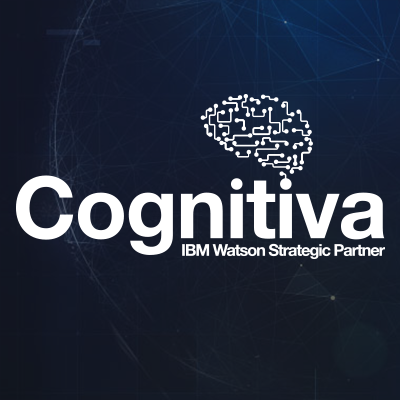
\includegraphics[width=.8\textwidth]{computacionCognitiva}
		\caption{Computaci\'on Cognitiva}
		\label{fig:computacionCognitiva}
	\end{center}
\end{figure}
		
    \item{Blockchain permitir\'a mayor veracidad y confianza en cadenas de valor a trav\'es de la nube:} El blockchain es una base de datos descentralizada en la red. Un sistema que permite que partes que no conf\'ian plenamente unas en otras puedan mantener consenso sobre distintas operaciones que se hagan entre ellas. As\'i que una blockchain es una red global de ordenadores que gestionan una gigantesca base de datos abierta al p\'ublico que se autorregula sin necesidad de ning\'un organismo central o persona. Cada vez son m\'as las empresas y organizaciones que est\'an optando por esta tecnolog\'ia, tendencia que continuar\'a en 2017.
		
		\begin{figure}[ht]
	\begin{center}
		
\includegraphics[width=.8\textwidth]{blockchain}
		\caption{Blockchain}
		\label{fig:blockchain}
	\end{center}
\end{figure}
		
    \item{Cloud computing va a facilitar la seguridad:} Con la inclusi\'on de nuevas tecnolog\'ias siempre surgen problemas de seguridad y a pesar de que la amenaza es real, los principales proveedores de nube est\'an tomando medidas extraordinarias para construir nuevos sistemas de seguridad. Y es aqu\'i donde la computación cognitiva tambi\'en juega un importante papel, pues en 2017, nuevas capacidades cognitivas acelerar\'an la transformaci\'on de las vulnerabilidades de seguridad percibidas de la nube. Generarán hip\'otesis, razonamiento basado en la evidencia y recomendaciones para mejorar la toma de decisiones. Como resultado, la seguridad cognitiva ayudar\'a a abordar la falta de capacidades actuales, acelerar las respuestas y ayudar a reducir el costo y la complejidad de hacer frente a la delincuencia inform\'atica.
		
		\begin{figure}[ht]
	\begin{center}
		
\includegraphics[width=.8\textwidth]{seguridad}
		\caption{Seguridad}
		\label{fig:seguridad}
	\end{center}
\end{figure}
		
    \item{La computaci\'on en nube “serverless” est\'a eliminando la complejidad y costo de desarrollo de aplicaciones:} Una tecnolog\'ia emergente llamada “computaci\'on sin servidor” hace que el uso de servidores virtuales y f\'isicos sea completamente invisible para los desarrolladores. Esta tecnolog\'ia, la cual es ofrecida en la nube, est\'a empezando a desentra\~nar las ventajas competitivas que cambian el juego para organizaciones de todos los tama\~nos, pues estas arquitecturas mitigan preocupaciones de parches de seguridad, control acceso y hacen un uso muy eficiente de los recursos de computaci\'on, adem\'as estos sistemas son f\'aciles de operar y ofrecen caracter\'isticas integradas de escalado. En 2017, m\'as empresas aprovechar\'an sus beneficios, incluyendo la reducci\'on del tiempo de desarrollo y costos m\'as bajos.
		
		\begin{figure}[ht]
	\begin{center}
		
\includegraphics[width=.8\textwidth]{serverless}
		\caption{Serverless}
		\label{fig:serverless}
	\end{center}
\end{figure}

		\item{La transformac\'on de la cultura est\'a impulsando el camino hacia la nube:} A medida que m\'as y m\'as organizaciones adoptan la nube, se requerir\'a una transformaci\'on que va m\'as all\'a de la tecnolog\'ia. Investigadores, desarrolladores, startups y organizaciones deben adoptar un cambio de cultura que priorice la experiencia del usuario y mejore la colaboraci\'on, la libertad para experimentar y un enfoque empresarial agudo. En 2017, vamos a ver m\'as empresas de TI que crear\'an espacios f\'isicos reales, como centros de innovaci\'on o garajes, donde el talento es atra\'ido y nutrido, y equipos pequeños podr\'an reunirse para aprender nuevas habilidades y colaborar en las innovaciones. Las plataformas en la nube acelerar\'an la innovaci\'on y el papel clave de la tecnolog\'ia de la informaci\'on en la transformaci\'on de los negocios y la sociedad.
		
		\begin{figure}[ht]
	\begin{center}
		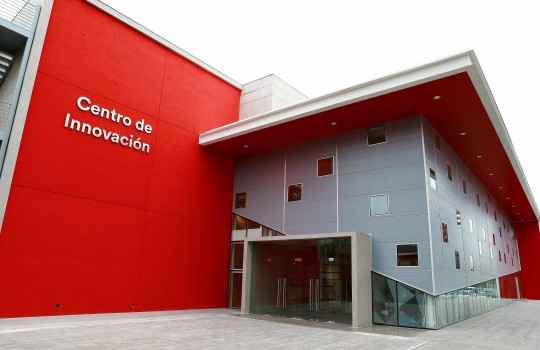
\includegraphics[width=.8\textwidth]{innovacion}
		\caption{Centros de innovaci\'on}
		\label{fig:innovacion}
	\end{center}
\end{figure}
\end{enumerate}

\end{justify}

%%%%%%%%%%%%%%%%%%%%%%%%%%%% CAPITULO 4 %%%%%%%%%%%%%%%%%%%%%%%%%%%%
\vspace*{5em}
\chapter{TECNOLOG\'IAS ACTUALES}
\vspace*{-2em}

Claramente la nube se est\'a convirtiendo en una plataforma de innovaci\'on y transformaci\'on general.
\\ Actualmente muchas empresas de todo el mundo est\'an ofreciendo una amplia gama de servicios en la nube, la abundancia puede ser abrumadora.
 
\section{Empresas que brindan servicios de Cloud}
\subsection{Amazon.com}
\begin{justify}
{\bf{Amazon Web Services (AWS)}} es una plataforma de servicios en la nube que ofrece potencia de c\'omputo, almacenamiento de bases de datos, entrega de contenido y otra funcionalidad para ayudar a las empresas a escalar y crecer. \citep{aws}

AWS se encuentra detrás del \'exito de muchas compañías, startups y sector p\'ublico, como: 
\begin{itemize}
	\item  \textbf{Netflix:} AWS permite a Netflix desplegar rápidamente miles de servidores y terabytes de almacenamiento en cuesti\'on de minutos. Los usuarios pueden ver programas y películas de Netflix desde cualquier parte del mundo, incluso en la web, en tabletas o en dispositivos móviles como el iPhone.\citep{awscasos}
	\item  \textbf{Spotify:}	Debido a que el objetivo de la compañía es ayudar a la gente a escuchar cualquier música que quieran, cuando quieran, Spotify se enfrenta al desaf\'io de catalogar no sólo ayer y las canciones populares de hoy, sino también todas las que se publicarán en el futuro. Spotify agrega más de 20.000 pistas al día a su catálogo. \\	
La  compa\~{n}\'ia cre\'o sistemas basados en Python para interactuar con su enorme volumen de contenido en Amazon S3. Además, Amazon CloudFront entrega la aplicación Spotify y las actualizaciones de software a los usuarios. \\ Al igual que las tendencias musicales cambian continuamente, Amazon Web Services (AWS) ayuda a Spotify a evaluar continuamente su infraestructura para cumplir con los objetivos de negocio en constante evoluci\'in.\citep{awscasos}
	\item  \textbf{Adobe:}Adobe utiliza AWS para proporcionar ambientes operativos de varios terabytes para sus clientes. Al integrar sus sistemas con AWS Cloud, Adobe puede centrarse en implementar y operar su propio software en lugar de infraestructura.\citep{awscasos}
\end{itemize}
De acuerdo con \cite{awscasos} otras  de las empresas que cuentan con el respaldo de AWS son  Dunkin Donuts, Airbnb, Kellogs, Siemens, BCP, Johmson-Johmson, etc. 
\\Actualmente la nube de AWS funciona en 44 zonas de disponibilidad dentro de 16 regiones geogr\'aficas del mundo, con planes anunciados para crear 14 zonas m\'as y cinco regiones adicionales en China, Francia, Hong Kong, Suecia y una segunda regi\'on AWS GovCloud en los EE.UU. \citep{aws}

\begin{figure}[ht]
\begin{center}
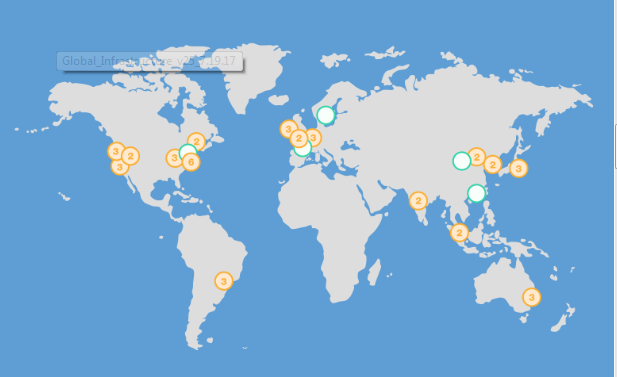
\includegraphics[scale=0.8]{aws_paises}
\end{center}
\begin{center}
\vskip -0.5cm
\caption{\small{Distribución de AWS.}}
{\small{Fuente: \cite{aws}}}
\end{center}
\end{figure}

\end{justify}
\subsection{Google Inc}
\begin{justify}
{\bf Google Cloud Plataform} consiste en un conjunto de servidores f\'isico as\'i como virtuales que est\'an contenidos en los centros de datos de Google alderedor del mundo.
\\ Google cuenta con el modo de despliegue  multi regional Google Cloud Plataform, lo cual permite al usuario elegir el centro de datos para sus aplicaciones.
\end{justify}
\begin{figure}[ht]
\begin{center}
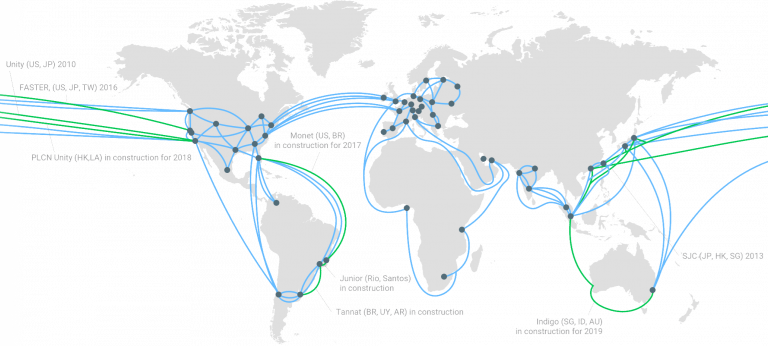
\includegraphics[scale=0.6]{google_cloud}
\end{center}
\begin{center}
\vskip -0.5cm
\caption{\small{Red de Google Cloud Platform.}}
{\small{Fuente: \cite{google_cloud}}}
\end{center}
\end{figure}
\begin{justify}
Según \cite{google_cloud} en las \'ultimas encuestas de SADA Systems sobre el uso p\'ublico de la nube, los  gerentes de TI encuestados dan se\~{n}ales del crecimiento que esta teniendo hoy en día la infraestructura de nube p\'ublica.
\end{justify}
\begin{figure}[ht]
\begin{center}
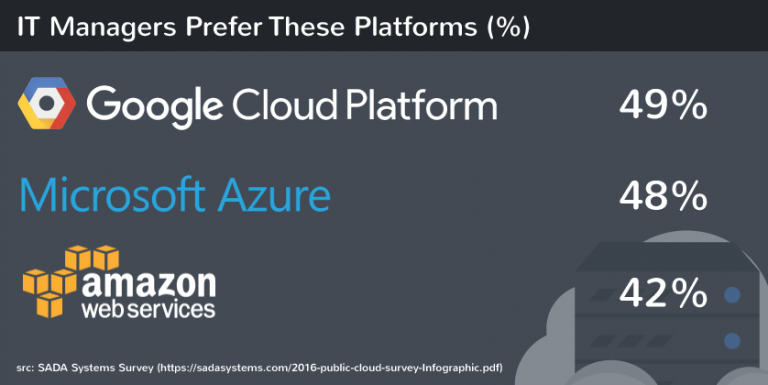
\includegraphics[scale=0.4]{encuesta}
\end{center}
\begin{center}
\vskip -0.5cm
\caption{\small{Resultados de Encuesta sobre el uso de nubes p\'ublicas}}
{\small{Fuente: \cite{google_cloud}}}
\end{center}
\end{figure}
\vskip 1.5cm
Estas son algunas de las empresas que  desarrollan sus productos con Google Cloud Platform:
\begin{itemize}
	\item \textbf{Pocket Gems:} Utiliza App Engine para procesar cientos de miles de jugadores m\'oviles en tiempo real.
	\item \textbf{Khan Academy :}Khan Academy usa Google Cloud Platform para poner cursos gratuitos y de gran calidad al alcance de todos.
	\item \textbf{Coca-Cola:} Comprueba cómo está utilizando Google Cloud Platform Coca-Cola para estar a la altura de los eventos deportivos más grandes del mundo.
	\item \textbf{Atomic Fiction:} Crea efectos especiales para las series de televisión y las películas más importantes del mundo, gracias a los potentísimos recursos informáticos de Google Cloud Platform.
\end{itemize}
\begin{justify}
Un gran punto a favor que tiene hoy en día Google Cloud Plataform es que permite la migraci\'on en vivo de m\'aquinas Virtuales, funcionalidad que ni Azure ni AWS tienen. En la siguiente figura se detallan los  pasos de alto nivel involucrados en una migración de VM en vivo (Figura \ref{migracion}).
\end{justify}
\FloatBarrier 
\begin{figure}[ht]
\begin{center}
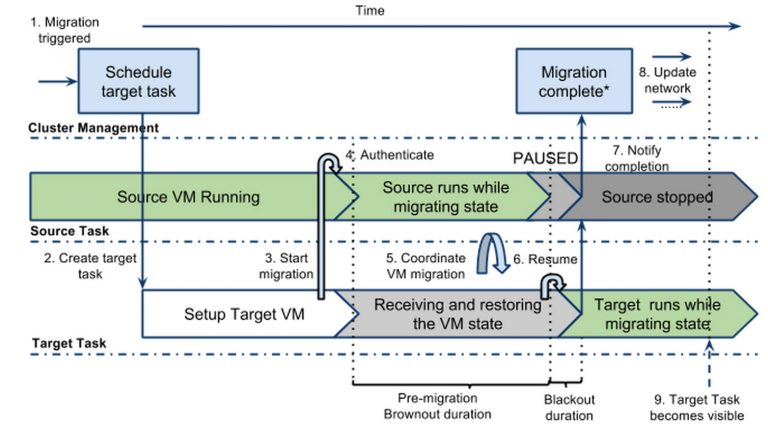
\includegraphics[scale=0.7]{migracion}
\end{center}
\begin{center}
\vskip -0.5cm
\caption{\small{ Pasos de alto nivel involucrados en una migraci\'on de VM en vivo}}
\label{migracion}
{\small{Fuente: \cite{google_cloud_migration}}}
\end{center}
\end{figure}

\subsection{Azure}
\begin{justify}
Microsoft Azure es una creciente colección de servicios en la nube integrados que los desarrolladores y los profesionales de TI utilizan para crear, implementar y administrar aplicaciones a través de nuestra red global de centros de datos. Con Azure, obtiene la libertad de crear e implementar donde quiera, utilizando las herramientas, las aplicaciones y los marcos que prefiera.\citep{azure_def}

Estas son algunas de las empresas que  desarrollan sus productos con Microsoft Azure:
\begin{itemize}
	\item \textbf{Carviresa :} Para mejorar la planificación y gestión de sus recursos, y centralizar los datos de negocio procedentes de sus tres ubicaciones.
	\item \textbf{Guzman Global :}La multinacional española ha elegido Microsoft Dynamics CRM Online por su usabilidad, escalabilidad y sus altos estándares de seguridad en la nube, factores que le permiten replicar su modelo fácilmente en diferentes países.
	\item \textbf{NAE :} Para mejorar su gestión comercial con la ayuda del partner Innovar Tecnologías.
\end{itemize}

\end{justify}
\newpage
\section{Casos de Implementación}
	\begin{justify}
	A continuación se presentarán  las diferentes que empresas o instituci\'on que aplicaron las buenas pr\'acticas en la implementaci\'on de diferentes soluciones cloud (Tabla \ref{tablaEmpresas}) , casos pertenecientes a diferentes ramas, actividad económica, administración publica, etc.
	\end{justify}

	\begin{table}[ht]		
		\centering
		\caption{Casos de \'Exito implementando Cloud Computing}
		\label{tablaEmpresas}
		\begin{tabular}{|p{4.2cm} |p{2.3cm} |p{2.5cm} |p{4cm}|} \hline
			\bf{Sector} & \bf{Proveedor} & \bf{Modelo de Negocio} & \bf{Empresa o Institución} 
			\\ \hline \hline
			Adminitraci\'on P\'ublica & Microsoft & SaaS &  Generalitat de Catalunya 
			\\ \cline{2-4}
			 & CIPSA y REGTSA & SaaS (cloud privada) & CIPSA y REGTSA  
			\\ \hline
			Audio Visuales  & Spotify & SaaS & AWS
			\\ \hline
			Correo electr\'onico & Amazon & PaaS / IaasS & AWS
			\\ \hline
			Inform\'atica y telecomunicaciones & Annova y Pixelware & PaaS & Proyecto PymeCloud 
			\\ \cline{2-4}
			 & EyeOS & PaaS & EyeOS  
			\\ \cline{2-4}
			 & Arsys & SaaS / PaaS / IaaS & EyeOS  
			\\  \cline{2-4}
			 & Fresh Books & SaaS & Fresh Books  
			\\  \hline
			Ivestigaci\'on, desarrollo y manufactura & Windows Azure & PaaS & 3M 
			\\ \hline
			Ivestigaci\'on Biom\'edica & VORTAL & SaaS & Organismo P\'ublico de España 
			\\ \hline
			Medios de Comuniaci\'on & NTS y Salesforce.com & SaaS & Grupo Vocento \\ \hline
			Transporte & Estudio Cero & SaaS & Estudio Cero\\ \hline 
		\end{tabular}
		\vskip 0.2cm
		\begin{center}
			{\small{Fuente: Elaboraci\'on Propia - \cite{Ferrari}.}}
		\end{center}
	\end{table}



\section{Diferencias entre Empresas que ofrecen Cloud Computing}
	\begin{justify}
	Seg\'un \cite{Akami} las empresas de Cloud Computing se diferencian seg\'un:
	\begin{enumerate}[label=\alph*)]
		\item \textbf{Tipo de servicio ofrecido: } En la nube existen diferentes tipos de servicio (v\'ease cap. \ref{cap1}. La entidad que se quiera contratar debe definir muy bien cu\'ales ser\'an los Acuerdos de Nivel de Servicio (SLA) que mejor se ajusten a las necesidades.
		\item \textbf{La escala y resistencia de la arquitectura:} Las mejores empresas de cloud computing tienen varios centros de datos dispersos geográficamente, lo que garantiza la disponibilidad ininterrumpida del servicio para sus cliente.
		\item \textbf{Calidad del componente de autoservicio:} La administraci\'on  de los servicios en la nube se realiza por un portal web, por ello, el portal debe contar con ciertas normas y permitir el control f\'acil del servicio.
		\item \textbf{Longevidad y experiencia:} Seg\'un \cite{CristianCA} en el 2012  el modelo de cloud computing se encontraba en etapa de desarrollo, por ese motivo existían pocas empresas que apostaban por el modelo; sin embargo,  en la actualidad existen cada día mas empresas ofreciendo este modelo, este es el motivo por el que cual al momento de querer adquirir los servicios que ofrece se debe tener en cuenta la experiencia, pues muchas son nuevas y no han sido probadas.
	\end{enumerate}
	Si desea conocer algunas recomendaciones para contratar servicios en la nube revise el documento de \cite{Beimar}
\end{justify}


%%%%%%%%%%%%%%%%%%%%%%%%%%%%%%%%%%%%%%%%%%%%%%%%%%%%%%%%%%%%%%%%%%%%%%%%%%%


\newpage
%%%%%%%%%%%%%%%%%%%%%%%%%%%% CONCLUSIONES %%%%%%%%%%%%%%%%%%%%%%%%%%%%
\addcontentsline{toc}{chapter}{Conclusiones}
\vspace*{6em}
\begin{center}
{\bf{\large{\underline{CONCLUSIONES}}}}
\end{center}
\begin{justify}
\begin{itemize}
    \item{}El mercado actual es muy competitivo y lo encabezan empresas que optan, principalmente, por este modelo, implementando ya sea una nube privada, pública o una híbrida. Esto debido a que una buena implementación mejora los servicios que ofrecen haciendo que los usuarios confien más y se popularice.
    \item{}Hoy en día las empresas siguen apostando por este modelo y seguirán surguiendo nuevos servicios y variaciones en estos. Por ello, si se quiere hacer uso de un servicio Cloud primero debemos analizar por completo los tipos y servicios que ofrece cada uno y ver cual se acomoda mejor al problema.
    \item{}La computación Cloud ha llegado para imponerse, aportando servicios que van aumentando significativamente de tal manera que cada dia más usuarios recurren para hacer uso de ellos.
    \item{}Es muy poco probable que, al hacer uso de los servicios de Computación Cloud, ocurran fallas o exista algún tipo de riesgo que afecte al negocio del contratador. Es por ello que este modelo es muy rentable.
\end{itemize}
\end{justify}
%%%%%%%%%%%%%%%%%%%%%%%%%%%%%%%%%%%%%%%%%%%%%%%%%%%%%%%%%%%%%%%%%%%%%%%%%%%



%%%%%%%%%%%%%%%%%%%%%%%%%%%% BIBLIOGRAFIA %%%%%%%%%%%%%%%%%%%%%%%%%%%%
\addcontentsline{toc}{chapter}{Bibliograf\'ia}
\vspace*{6em}
 \bibliography{Bibliografia}
%%%%%%%%%%%%%%%%%%%%%%%%%%%%%%%%%%%%%%%%%%%%%%%%%%%%%%%%%%%%%%%%%%%%%%%%%%%



\end{document}
